\problemname{Longest increasing pub-sequence}
\noindent

Elise has just started at Stackköping Institute of Technology (SIT), and as part of the reception a traditional pub crawl is organized.
A pub crawl involves visiting all student chapter halls and drinking something at each place.
Elise and her friends do not drink alcohol, but they do enjoy walking long distances.
Therefore, they plan to design a route with as many visits as possible, such that the distances they walk between the halls are strictly increasing.
Your task is to find the maximum number of visits they can achieve.

The student chapter halls are located at points in the plane with integer coordinates.
Elise and her friends always walk the shortest distance between two halls.
The distance is the usual Euclidean distance, i.e.\ $\sqrt{(x_1 - x_2)^2 + (y_1 - y_2)^2}$.
They may start at any hall.
It is allowed to visit the same hall multiple times, and each visit counts as a separate visit.
However, they may not visit the same place twice in a row.

\begin{figure}[!h]
\begin{center}
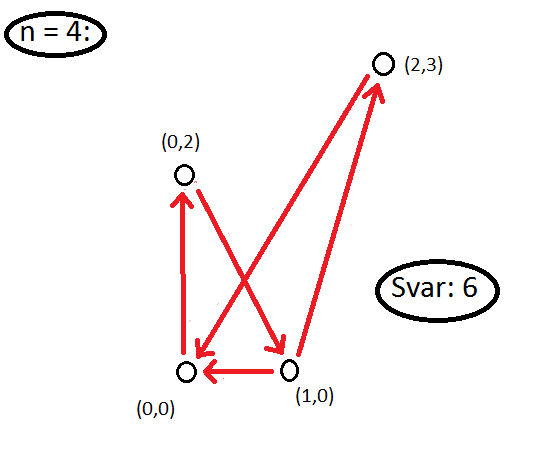
\includegraphics[width=8cm]{pubsequence.png}
\end{center}
\caption{The image shows Sample 1. If you start at $(1,0)$ and follow the red arrows, you get a route with $6$ visits, which is also the maximum.}
\end{figure}

\section*{Input}
The first line contains an integer $N$ ($2 \leq N \leq 2000$), the number of student chapter halls.
The following $N$ lines contain two integers $x_i, y_i$ ($0 \leq x_i, y_i \leq 10^9$), the coordinates for each hall.

\section*{Output}
Print a single integer, the maximum number of visits Elise and her friends can make if the distances between consecutive points are strictly increasing.

\section*{Scoring}
Your solution will be tested on a set of test groups.
To earn points for a group, you must pass all test cases in that group.

\noindent
\begin{tabular}{| l | l | l |}
\hline
Group & Points & Constraints \\ \hline
$1$    & $10$         & $N \leq 3$ \\ \hline
$2$    & $10$         & $N \leq 5$ \\ \hline
$3$    & $30$         & $N \leq 200$ \\ \hline
$4$    & $50$         & No additional constraints \\ \hline
\end{tabular}
